\section{\texorpdfstring{Ukázka komunikace}{Ukazka komunikace}}

% =====================================================================================================================
	\begin{frame}
    \frametitle{Zadání}
		
		\begin{itemize}
			\item Vytvořit python skript zajišťující spuštění modbus TCP serveru (\textcolor{red}{\textbf{pozor, toto je slave !!!}}),
			\item server bude mít lokální přístup na IP adrese 127.0.0.1:502,
			\item server bude poskytovat následující data:
			
			\begin{itemize}
				\item fyzická adresa 0 až 4 pro cívky, volně nastavitelný stav,
				\item fyzická adresa 0 až 4 pro digitální vstupy, náhodně měnící se stav,
				\item fyzická adresa 0 až 4 pro vstupní registry, náhodně měnící se hodnota,
				\item fyzická adresa 0 až 4 pro uchovávací registry, volně nastavitelná hodnota,
			\end{itemize}
			
			\item server bude otestován programem QModMaster.
		\end{itemize}
		
	\end{frame}
	
% =====================================================================================================================
	\begin{frame}
    \frametitle{Zadání}
		
		\begin{itemize}
			\item Vytvořit python skript zajišťující spuštění modbus TCP serveru (\textcolor{red}{\textbf{pozor, toto je slave !!!}}),
			\item server bude mít lokální přístup na IP adrese 127.0.0.1:502,
			\item server bude poskytovat následující data:
			
			\begin{itemize}
				\item fyzická adresa 0 až 4 pro cívky, volně nastavitelný stav,
				\item fyzická adresa 0 až 4 pro digitální vstupy, náhodně měnící se stav,
				\item fyzická adresa 0 až 4 pro vstupní registry, náhodně měnící se hodnota,
				\item fyzická adresa 0 až 4 pro uchovávací registry, volně nastavitelná hodnota,
			\end{itemize}
			
			\item server bude otestován programem QModMaster.
		\end{itemize}
		
	\end{frame}

% =====================================================================================================================
	\begin{frame}
    \frametitle{Python skript - data}
		
		\begin{center}
			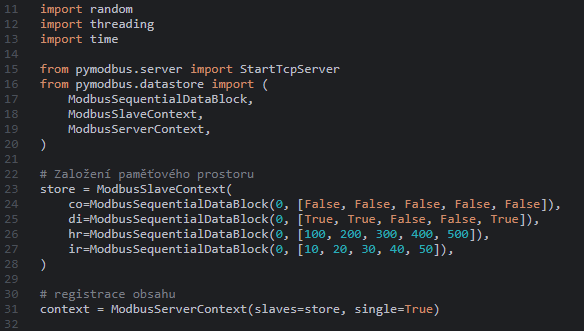
\includegraphics[width=0.90\textwidth]{fig/python_ukazka_data.png}
		\end{center}
		
	\end{frame}

% =====================================================================================================================
	\begin{frame}
    \frametitle{Python skript - vlákna}
		
		\begin{center}
			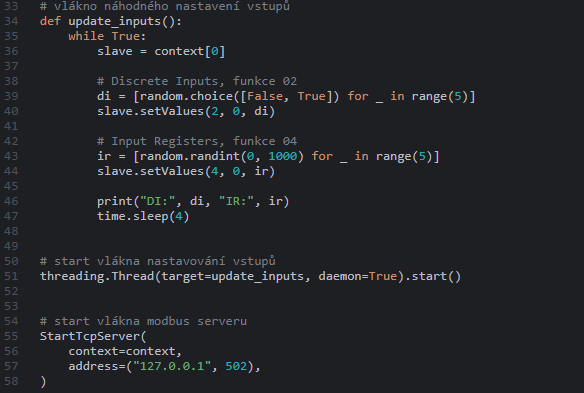
\includegraphics[width=0.90\textwidth]{fig/python_ukazka_vlakna.png}
		\end{center}
		
	\end{frame}
	
% =====================================================================================================================
	\begin{frame}
    \frametitle{QModMaster - nastavení IP adresy serveru}
		
		\begin{center}
			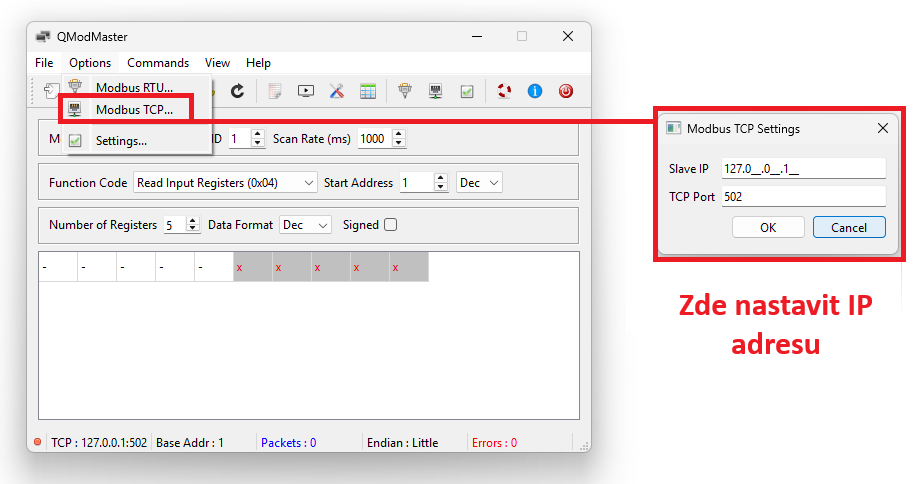
\includegraphics[scale=0.40]{fig/qmod_ipadr.png}
		\end{center}
		
	\end{frame}
	
% =====================================================================================================================
	\begin{frame}
    \frametitle{QModMaster - ovládání}
		
		\begin{center}
			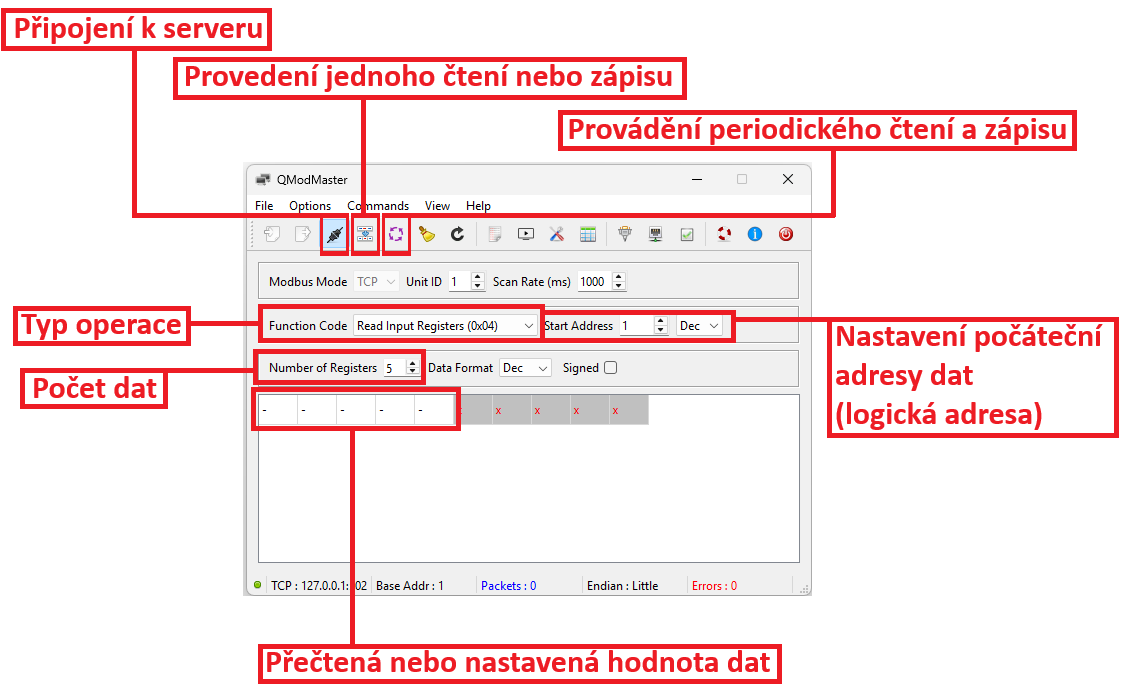
\includegraphics[scale=0.40]{fig/qmod_ovl.png}
		\end{center}
		
	\end{frame}
	
% =====================================================================================================================
	\begin{frame}
    \frametitle{QModMaster - monitor}
		
		\begin{center}
			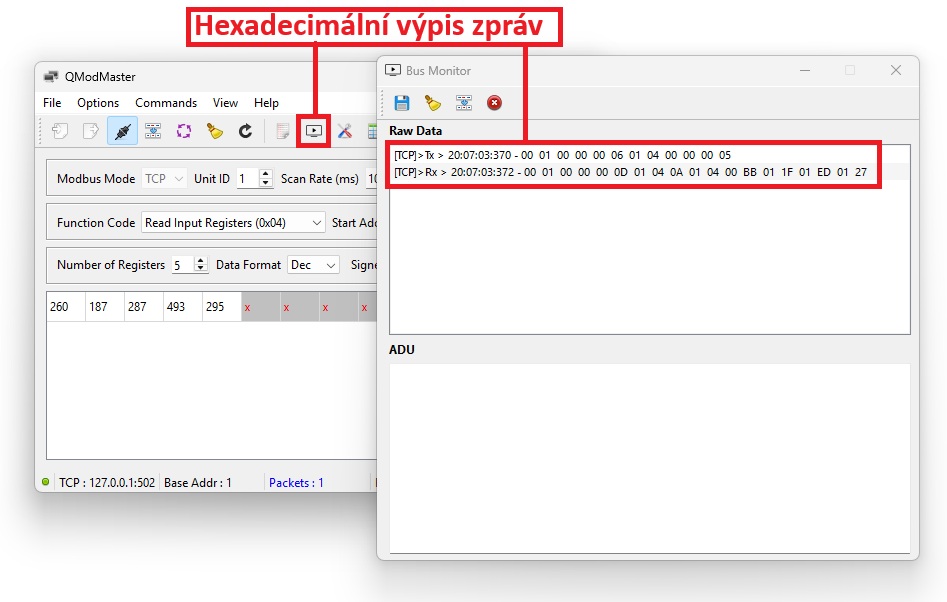
\includegraphics[scale=0.40]{fig/qmod_mon.png}
		\end{center}
		
	\end{frame}
	
% =====================================================================================================================
	\begin{frame}
    \frametitle{QModMaster - k vyzkoušení}
		
		\begin{itemize}
			\item zápis nebo čtení od adresy 1 více jak 5 a méně jak 9 binárních dat, 
			\item zápis nebo čtení od adresy 1 více jak 8 binárních dat, 
			\item zápis nebo čtení od adresy 1 více jak 5 číselných dat.
		\end{itemize}
		
	\end{frame}